\StartPlate{V01}{The three obligations}{Finite comparison, arithmetic existence, and characterization have different inputs.}
\begin{center}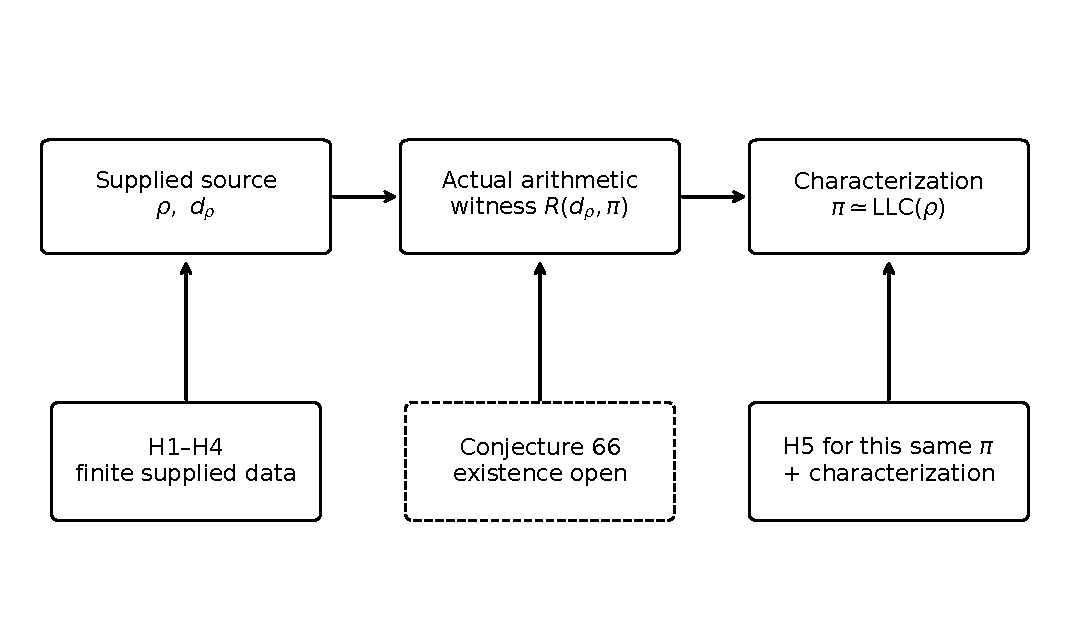
\includegraphics[width=\linewidth]{figures/V01.pdf}\end{center}
The source is a wild Weil atom $\rho$ with the supplied datum $d_\rho$. H1--H4 include the declared finite break decomposition, symplectic bridges, central extensions and phases, and coherent transports. They describe an admitted input. They do not assert that every possible source arrives with canonical data.

The middle box is an actual arithmetic witness $R(d_\rho,\pi)$. It carries the prescribed packet and recovers the same supercuspidal representation, including the central character and noncompact completion. The final arrow additionally needs H5 for that particular $\pi$ and the applicable characterization theorem.
\[
\forall\rho\in\mathcal A\quad\exists\pi\;R(d_\rho,\pi)
\qquad\hbox{is the general realization endpoint.}
\]
An arrow is a dependency, not a declaration that its input has been constructed. Restricted witnesses and finite comparison theorems remain useful even while this quantified endpoint is open. Historical obligation 66 is not a measure of the amount of mathematics still required.
\vfill\PlateSource{Contract diagram}{Part I, Section 1}{6}
